\documentclass[12pt]{article}
\usepackage[margin=1in]{geometry}
\usepackage{graphicx}
\usepackage{listings}
\usepackage{parskip}

\lstdefinestyle{mystyle}{
    basicstyle=\ttfamily\footnotesize,
    breakatwhitespace=false,         
    breaklines=true,                 
    captionpos=b,                    
    keepspaces=true,                 
    numbers=left,                    
    numbersep=5pt,                  
    showspaces=false,                
    showstringspaces=false,
    showtabs=false,                  
    tabsize=2
}

\lstset{style=mystyle}

% copied from riscv-isa-manual
\usepackage{longtable}
\usepackage{multirow}
\usepackage{array}


% Commands for register format figures.

% New column types to use in tabular environment for instruction formats.
% Allocate 0.18in per bit.
\newcolumntype{I}{>{\centering\arraybackslash}p{0.18in}}
% Two-bit centered column.
\newcolumntype{W}{>{\centering\arraybackslash}p{0.36in}}
% Three-bit centered column.
\newcolumntype{F}{>{\centering\arraybackslash}p{0.54in}}
% Four-bit centered column.
\newcolumntype{Y}{>{\centering\arraybackslash}p{0.72in}}
% Five-bit centered column.
\newcolumntype{R}{>{\centering\arraybackslash}p{0.9in}}
% Six-bit centered column.
\newcolumntype{S}{>{\centering\arraybackslash}p{1.08in}}
% Seven-bit centered column.
\newcolumntype{O}{>{\centering\arraybackslash}p{1.26in}}
% Eight-bit centered column.
\newcolumntype{E}{>{\centering\arraybackslash}p{1.44in}}
% Ten-bit centered column.
\newcolumntype{T}{>{\centering\arraybackslash}p{1.8in}}
% Twelve-bit centered column.
\newcolumntype{N}{>{\centering\arraybackslash}p{2.02in}}
% Fifteen-bit centered column.
\newcolumntype{M}{>{\centering\arraybackslash}p{2.2in}}
% Sixteen-bit centered column.
\newcolumntype{K}{>{\centering\arraybackslash}p{2.88in}}
% Twenty-bit centered column.
\newcolumntype{U}{>{\centering\arraybackslash}p{3.6in}}
% Twenty-bit centered column.
\newcolumntype{L}{>{\centering\arraybackslash}p{3.6in}}
% Twenty-five-bit centered column.
\newcolumntype{J}{>{\centering\arraybackslash}p{4.5in}}


\newcommand{\instbit}[1]{\mbox{\scriptsize #1}}
\newcommand{\instbitrange}[2]{~\instbit{#1} \hfill \instbit{#2}~}

\newcommand{\wiri}{\textbf{WIRI}}
\newcommand{\wpri}{\textbf{WPRI}}
\newcommand{\wlrl}{\textbf{WLRL}}
\newcommand{\warl}{\textbf{WARL}}

% end of copied from riscv-isa-manual

\newcommand{\note}{\vspace{1em}\textbf{NOTE: }}
\newcommand{\noteend}{\vspace{1em}}
\newcommand{\consider}{\textbf{CONSIDER: }}

\newcommand{\idWidth}{{6}}
\newcommand{\iommucap}{\textit{iommucap}}
\newcommand{\iommucapen}{\textit{iommucapen}}
\newcommand{\rsidlen}{\textit{RSIDLEN}}
\newcommand{\rsiddiv}{\textit{rsiddiv}}
\newcommand{\ersiddiv}{\textit{ersiddiv}}
\newcommand{\dtbase}{\textit{dtbase}}
\newcommand{\iommucause}{\textit{iommcause}}
\newcommand{\ftval}{\textit{ftval}}
\newcommand{\ftdevid}{\textit{ftdevid}}
\newcommand{\invltlb}{\textit{invltlb}}
\newcommand{\iommucfg}{\textit{iommucfg}}
\newcommand{\resume}{\textit{resume}}
\newcommand{\resumetype}{\textit{resumetype}}
\newcommand{\iommuintno}{\textit{iommuintno}}
\newcommand{\iommuinten}{\textit{iommuinten}}
\newcommand{\dtlen}{\textit{DTLEN}}
\newcommand{\dte}{\textit{dte}}


\begin{document}

\title{Xuantie IOMMU Specification Version 1.0 (Draft)}
\author{Siqi Zhao}
\maketitle


This document describes an IOMMU design specification for the Xuantie platform, which is
based on harts of the RISC-V architecture.

An IOMMU is used to translate virtual addresses in DMA requests from external devices
connected on certain peripheral bus to physical addresses. Abstractly, for all addresses
that can be accessed by an entity identified by a source ID, the IOMMU maintains a relation
from the tuple (source ID, virtual address) to a physical address.

The source ID identifies the entity that initiates DMA operations. The exact meaning of
the entity is dependent on the peripheral bus that the IOMMU is
interfaced with. For example, when the IOMMU is used to translate virtual addresses from
a PCI-Express device, the entity may refers to the \textit{device functions} in the
PCI-Express device. For simplicity, the rest of this document refers to such an entity as
a device. It is also assumed that one device is only capable of generating DMA operations
tagged with one unique identifier.

\note It is up to the implementation to define the exact entity that the term 'device'
refers to. \noteend

The IOMMU utilizes a table structure to maintain the aforementioned
mapping relation. The table structure could be implemented as register arrays or as memory
resident data structure. The table structure consists of multiple levels of tables. There are two
types of tables, the upper levels are IOMMU-specific look-up tables indexed by the source
IDs. The lower level tables contain entries that are the same as the page table entries as
defined in the RISC-V privileged architecture.

\note Typically, peripheral devices assigned to a virtual machine can also send interrupts
that target the harts of that virtual machine, and these interrupts need to be routed as
well, however, this design only specifies the DMA address translations. For interrupts,
the Advanced Interrupt Architecture (AIA) already includes the capability to redirect
interrupts from the devices to specific harts.\noteend

The address translation can be performed with either one stage or two stages. An operating
system kernel may utilize one-stage translation to directly assigned a device to a
process. A hypervisor may utilize the second stage of the two-stage translation to assign
a device to a virtual machine (VM), while the kernel in the VM may utilize the first stage
to further assign the device to processes. Any stage of the translation can be identity
mapping, i.e., no translation in effect.

The IOMMU can optionally implement a translation buffer that caches recent translation
entries. 

\section{System Architecture}
\label{sec:sys_arch}

The IOMMU is designed to be flexible and adaptive so that it is possible to integrate it
into various system architecture. The IOMMU works transparently between the peripheral bus
and the memory.

In a transparent configuration, the peripheral bus is not aware of the existence of the
IOMMU. The IOMMU transparently performing address translation for the memory access
requests from the peripheral bus. This configuration is intended for easy integration with
existing systems. This configuration is illustrated by Figure \ref{fig:trans-conf}.

\begin{figure}[ht!]
    \centering
    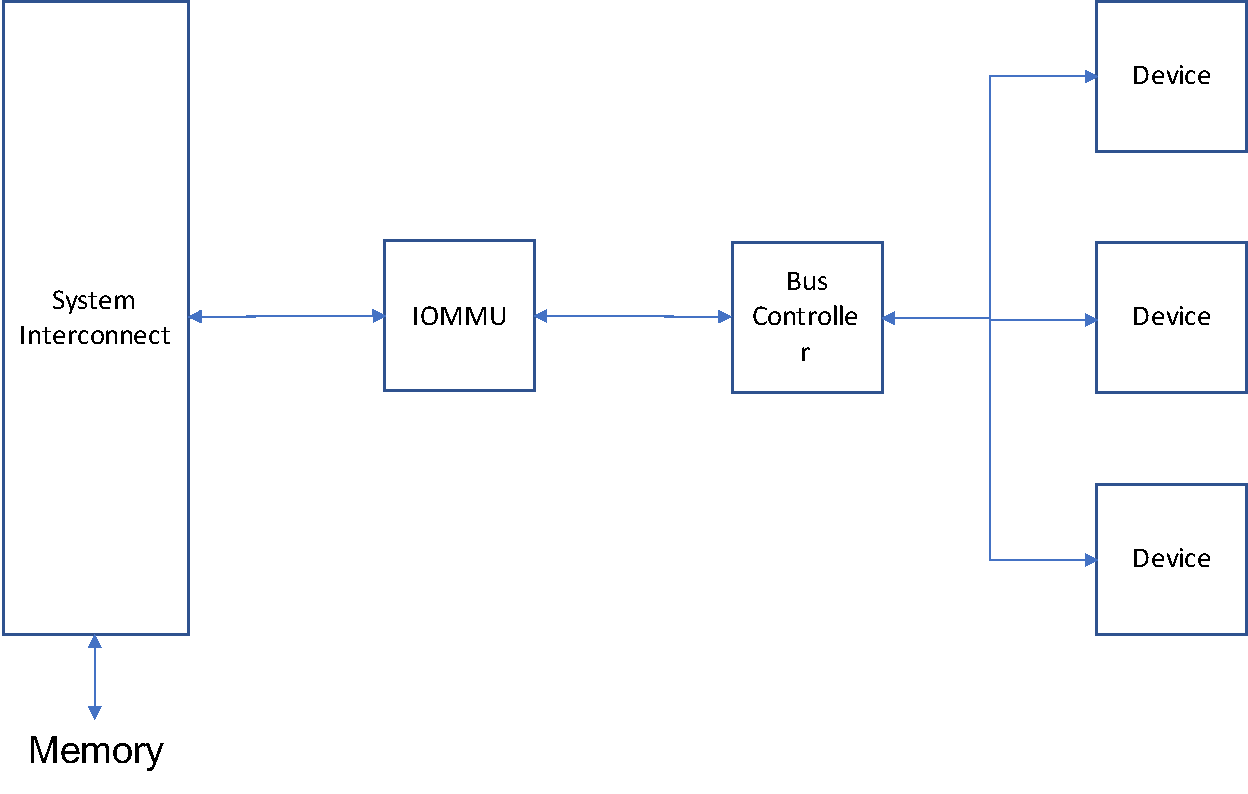
\includegraphics[width=0.95\textwidth]{img/trans-conf.pdf}
    \caption{Transparent Configuration of the IOMMU}
    \label{fig:trans-conf}
\end{figure}


\section{Interface}

At a high-level, the IOMMU exposes two interfaces. The CPU interface is for the
configuration and control of the IOMMU by the CPUs. The bus interface is for interacting
with the bus controllers. The bus interface accepts \textit{translation requests} and
returns translated addresses or faults.

\subsection{CPU Interface}

There are two 4K-aligned MMIO regions (the sizes are to be decided), one for accessing
translation-related register, called the \textit{register MMIO range}. The other is meant
for controlling the runtime behavior of the IOMMU, called the \textit{command MMIO range}.

The rationale of this divided regions is that some registers ('data registers') contain
data that the IOMMU utilize to carry out its function, mainly address translation.
Meanwhile, other registers ('control registers') act as 'triggers' in the sense that they
do not provide runtime data, instead they initiate certain operations of the IOMMU. This
separation facilitates the emulation of the IOMMU, so that the data registers can be
emulated by memory, which the control registers can be emulated by exceptions.

\subsubsection{Feature Discovery}

The IOMMU provides a register called \iommucap\ to allow harts to discover implemented
IOMMU features. The following bits are defined.

\begin{enumerate}
    \item S  bit: if S = 1, stage-two translation is implemented.
\end{enumerate}

\subsubsection{Feature Enable / Disable}

The IOMMU provides a register called \iommucapen\ to allow harts to enable or disable
certain features. The following bits are defined.

\begin{enumerate}
    \item E bit: if E = 1, the IOMMU is active. If E = 0, the IOMMU is inactive, all
        addresses in the memory requests are treated as physical addresses.
\end{enumerate}

\subsection{Bus Interface}

The underlying physical link with the peripheral bus that the IOMMU is working with is
\textit{implementation defined}. This link usually specifies the topology, command
interface and transport protocol with respect to utilizing the translation service of
the IOMMU.

An example is that for an on-chip AXI bus, the IOMMU sits between the bus masters and the
system interconnect, and by default translate all DMA requests from devices on the bus.

The IOMMU manages address translation on a per-device basis. For each device, the system
software can choose to setup address translation or configure it to be in the bypass mode
that directly works with physical addresses. 

The devices' memory accesses are treated as a sequence of transactions. Each transaction
may contain more than one transfer operation on the bus. The IOMMU works with
transactions, considering all addresses and data transferred within one transaction as a
whole group.

The IOMMU expects that the address range in the transactions adheres to restrictions
imposed by the bus protocol of that device. Typically, such restrictions limit the range
to within a 4K-aligned range, which is the minimum page size supported by the IOMMU. The
IOMMU does not perform more than one translation for each memory transaction. When the
IOMMU receives a transaction whose address range exceeds such limitation, it signals
failure to the device immediately.
% This limitation can be alleviated by using larger page sizes. %

The IOMMU does not affect the caching and ordering part of the peripheral bus protocol, if
any.

\subsection{Components and Placement}

The architecture presented in Section \ref{sec:sys_arch} illustrates the high-level
concept of the IOMMU's role in the whole system. Actual hardware implementation does not
need to strictly follow the illustration. In fact, depending on the requirement, a system
may choose to present a view of the IOMMU configuration different from the actual hardware
implementation. For example, a system may choose to configure the devices in the following
manner: assigning one IOMMU for one device and arranging for multiple device to share
another IOMMU, as illustrated in Figure \ref{fig:cmp_plcmnt}

\begin{figure}[ht!]
    \centering
    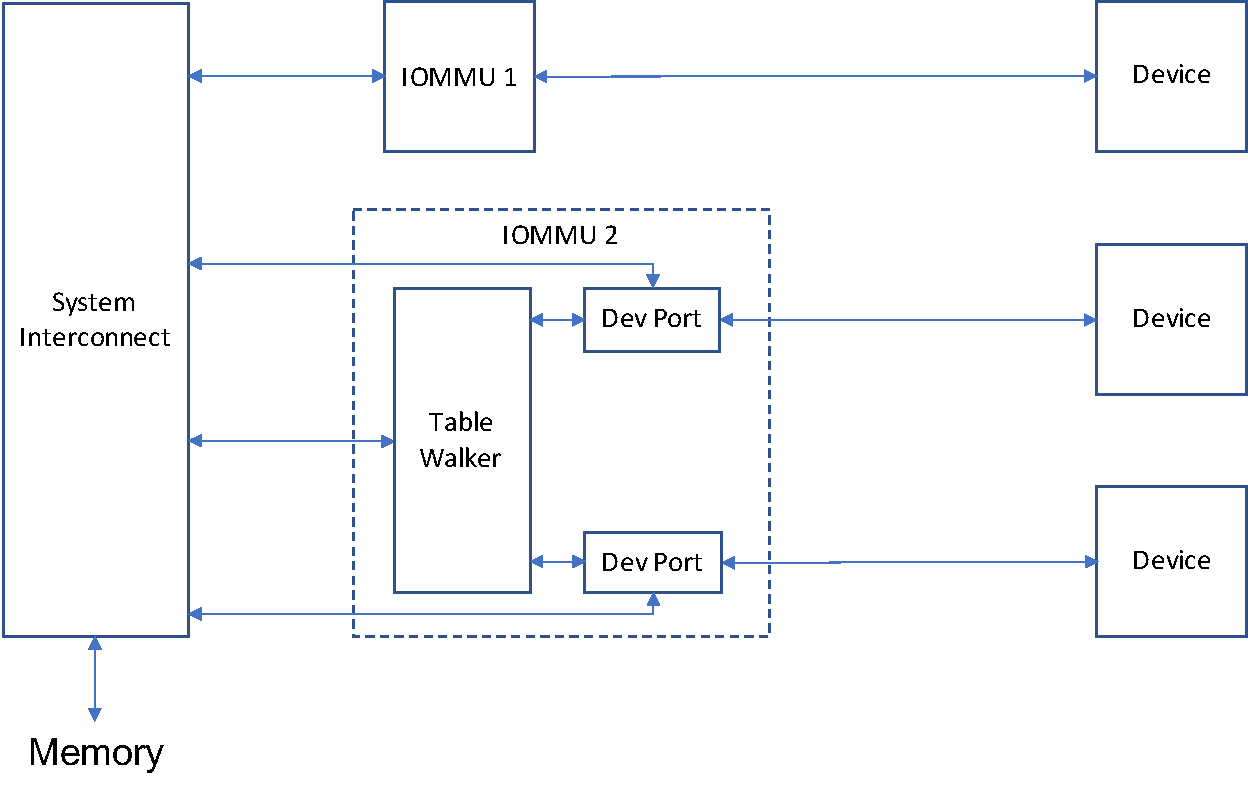
\includegraphics[width=0.95\textwidth]{img/cmp_plcmnt.pdf}
    \caption{An Example Configuration}
    \label{fig:cmp_plcmnt}
\end{figure}

However, the underlying hardware implementation can be very different. The dedicated IOMMU
may be a monolithic unit. Meanwhile, the shared IOMMU consists of sub-modules such as
device ports, translation table walker and buffers and caches. The implementation is
free to incorporate custom means to coordinate the operations of the sub-modules. However,
the components as a whole is logically exposed as one IOMMU.

It is possible for multiple IOMMU to collaborate. For example, one dedicated IOMMU may be
'dumb' and merely consists of a number of buffered translation entries. On a buffer miss,
this IOMMU requests address translation from another fully-featured IOMMU and obtains
translation results. This two IOMMUs are implemented differently, however, for some
specific reason from the platform, they are logically exposed as two functionally
equivalent IOMMU. Obviously, the necessary interaction between IOMMUs in this example is
\textit{implementation defined}. Figure \ref{fig:collab} illustrates this situation.

\begin{figure}[ht!]
    \centering
    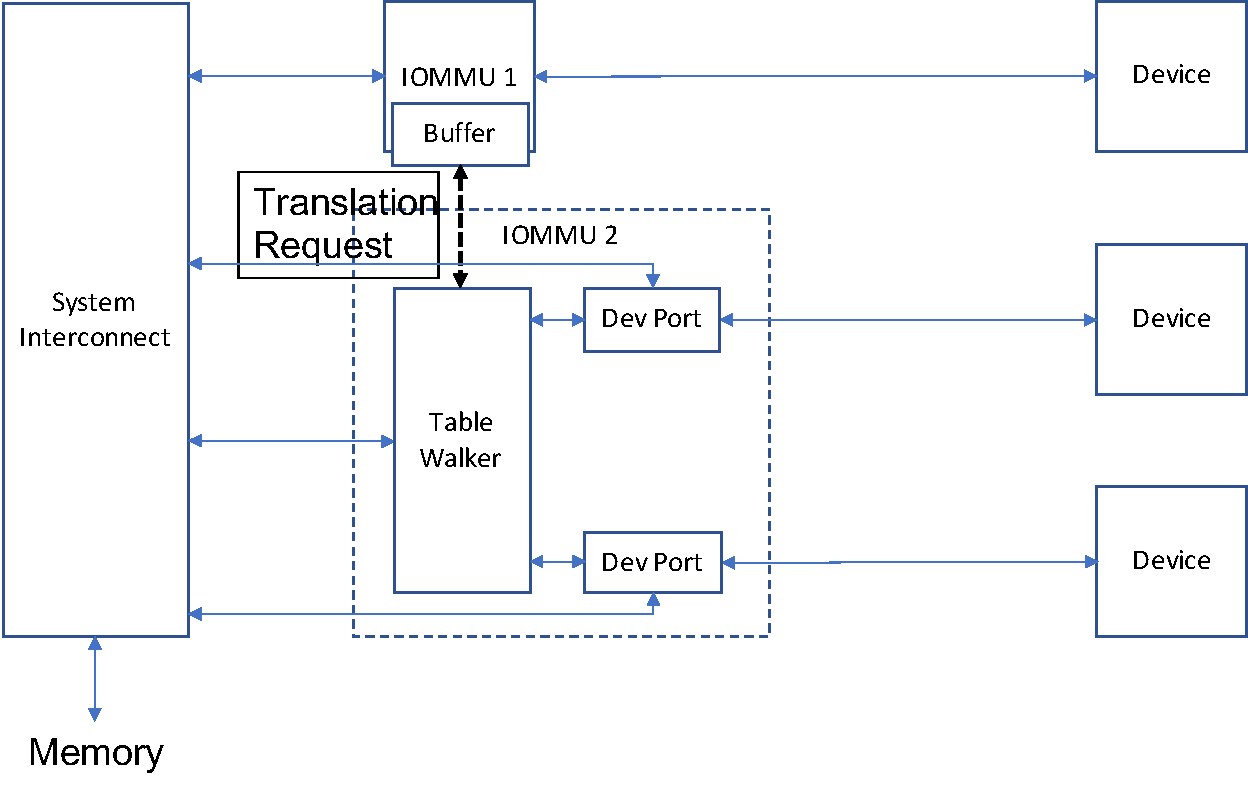
\includegraphics[width=0.95\textwidth]{img/collab.pdf}
    \caption{IOMMU Collaboration}
    \label{fig:collab}
\end{figure}




\section{Device Configuration}

Abstractly, the IOMMU uses a set of table structure to configure address translation
for individual devices. This table structure is collectively referred to as the
\textit{Device Tables}.

It is up to the implementation to determine whether the device tables are memory-resident
or stored in special registers provided by the IOMMU. When the device tables are stored in
specialized registers, the registers should be MMIO register and the MMIO registers should
reside in the register MMIO range of the IOMMU. In this case, the register \dtbase\ is not
defined.

Each IOMMU is associated with a \textit{domain} which consists of the devices whose DMA
requests is translated by this IOMMU. Each device within the same domain is assigned a
unique identifier, typically by the peripheral bus. The identifier is used to tag the relevant
memory requests originated from that device. Upon receiving the memory requests, the IOMMU
looks up in the device tables using the identifier and retrieve the configuration for that
device.

The identifier for the incoming translation requests is termed a Requester Source ID
(RSID). The length of the RSID is \rsidlen.

\subsection{Source Identification}

The RSID is split into two parts for use in the device table look-up, RISDHI and
RSIDLO. The MMIO register called \rsiddiv\ specifies the split point. When \rsiddiv\ stores
value $N$, RSIDLO is RSID[$N-1$:$0$] and RSIDHI is RSID[$\rsidlen - 1$, $N$]. The
\rsiddiv\ register is \warl, an implementation can hardwire this register to a fixed
value. When \rsiddiv is zero, RSIDHI equals RSID and RSIDLO is not defined.

The \rsidlen\ is implementation defined. It should be at least such a length so that it is
capable to contain the all the IDs of the bus that the IOMMU is intended to work with.

\note The RSID corresponds to the identification in the bus that it is interfaced with.
For example, the AXI bus assigns an ID to each device, and each device is capable of
generating transactions of possibly multiple IDs. The concatenated ID is the RSID. In this
case the RSID should be at least as long as the concatenated ID.\noteend

\note In the case of AXI, the RSID is not the transaction ID. \noteend


\subsection{Device Table}
\label{sec:dev_tbl}

\subsubsection{Memory Resident Device Table}
\label{sec:mem_dt}

The device tables are 8-byte aligned arrays of 8-byte aligned entries called
\textit{device table entries}.

When \rsiddiv\ is not zero, there are two levels of device tables. The level-1 device
tables are indexed by RSIDHI, and the level-2 device tables are indexed by RSIDLO. The
level-1 device table entries contains the base address of the corresponding level-2 device
table. The level-2 device table entries point to \textit{translation descriptors} for that
device with the RSID that leads to the entry.  The translation descriptor contains the
base address of the top level page table and other control bits.

When \rsiddiv\ is zero, there is only one level of device table index by RSID. The entries
point to the translation descriptor for that device with the RSID.

If the IOMMU implements the memory resident device table support, it provides an
MMIO register called \dtbase\ that holds the 8-byte aligned physical address of the
level-1 device table in the memory. The \dtbase\ register resides in the register MMIO
range.

The \dtbase\ register is defined in Figure \ref{fig:dtbase_reg}. 

\begin{figure}[h!t]
    \begin{center}
        \begin{tabular}{@{}Jc@{}F}
    \instbitrange{63}{3} &
    \instbitrange{2}{0} \\
    \hline
    \multicolumn{1}{|c|}{Addr} &
    \multicolumn{1}{c| }{Reserved} \\
    \hline
    61 & 3 \\

    \end{tabular}
    \end{center}

    \caption{dtbase Register}
    \label{fig:dtbase_reg}
\end{figure}

The Addr field store the 8-byte aligned physical address of the level-1 device table.

When \rsiddiv\ is not zero, the device tables are multi-level structures. The level-1
device table contains $2^{RSIDHI}$ entries that points to level-2 tables. The level-1
device table is index by RSIDHI derived from the RSID. The level-1 device table entries
are defined in Figure \ref{fig:lv1_dt_entry}.

\begin{figure}[h!t]
    \begin{center}
        \begin{tabular}{@{}Jc@{}F}
    \instbitrange{63}{3} &
    \instbitrange{2}{0} \\
    \hline
    \multicolumn{1}{|c|}{Addr} &
    \multicolumn{1}{c| }{Reserved} \\
    \hline
    61 & 3 \\

    \end{tabular}
    \end{center}

    \caption{Level-1 Device Table Entry}
    \label{fig:lv1_dt_entry}
\end{figure}

The Addr field store the 8-byte aligned physical address of the level-2 device table.

The Reserved bits must be zero, otherwise the IOMMU raises a fault.

The level-2 device tables are 8-byte aligned tables indexed by RSIDLO. Each table contains
$2^{RSIDLO}$ entries that points to an extended device table. The level-2 device table
entries are defined in Figure \ref{fig:lv2_dt_entry}.

\begin{figure}[h!t]
    \begin{center}
        \begin{tabular}{@{}Jc@{}I@{}I@{}I}
    \instbitrange{63}{3} &
    \instbit{2} &
    \instbit{1} &
    \instbit{0} \\
    \hline
    \multicolumn{1}{|c|}{Addr} &
    \multicolumn{1}{c| }{F} &
    \multicolumn{1}{c| }{S} &
    \multicolumn{1}{c| }{V} \\
    \hline
    61 & 1 & 1 & 1 \\

    \end{tabular}
    \end{center}

    \caption{Level-2 Device Table Entry}
    \label{fig:lv2_dt_entry}
\end{figure}

The Addr field store the 8-byte aligned address of the translation descriptor.

The V bit controls if the address translation is enabled for the particular device
identified by the RSID. If V bit is set, the address translation is in effect i.e. the
address in the transaction from the originating device is subject to translation. If V bit
is clear, the address translation for that device is turned off, i.e. the IOMMU forwards
the address as-is.

The S bit controls whether the device whose RSID leads to the level-2 device table entry
is subject to two-stages of address translation. If S bit is set, it is subjected to
two-stages of translation. If S bit is clear, it is only subject to one-stage of
translation.

The F bit controls whether the device whose RSID leads to the level-2 device table entry
is subject to stage-one address translation. If F bit is set, stage-one address
translation is enabled. If F bit is cleared, stage-one address translation is disabled,
i.e., the address in the DMA transaction is used only with stage-two address translation.

When \rsiddiv\ is zero, there is only one level of device table. The entries in the
level-1 device table are the same as the level-2 device table when \rsiddiv\ is not zero.

\subsubsection{Register-based Device Table}

If the device tables are implemented as MMIO registers, the IOMMU provides $2^\rsidlen$ number
of registers called \dte[$x$], where $0 <= x <= 2^\rsidlen - 1$. The format of the register is
shown in Figure \ref{fig:dtex}. 
The upper bits
beyond the width of the physical address on the hardware platform can be ignored.

The IOMMU does not support stage-two translation if the device tables are implemented as
MMIO registers.

\begin{figure}[h!t]
    \begin{center}
        \begin{tabular}{@{}J@{}I@{}I}
    \instbitrange{63}{2} &
    \instbit{1} &
    \instbit{0} \\
    \hline
    \multicolumn{1}{|c|}{Addr} &
    \multicolumn{1}{c| }{P} &
    \multicolumn{1}{c| }{V} \\
    \hline
    61 & 1 & 1 \\

    \end{tabular}
    \end{center}

    \caption{Device Table Entry Implemented as MMIO Register}
    \label{fig:dtex}
\end{figure}

The Addr field stores the base address of the top level address table for the device with
the RSID. The P bit indicates the fault reporting mode of the device. If P bit is set, the
IOMMU suspend the in-flight transaction that caused a fault. If P bit is cleared, the
IOMMU terminates the transaction immediately. 

If the V bit is set, the device table entry is valid. Otherwise, the entry is invalid.

The \dte[$x$] registers reside in a dedicated 4K-aligned region called device table range.

The IOMMU uses the content of \dte[$x$] for the device with RSID value $x$ to get the
address of the translation descriptor. The IOMMU zero-extend the content of the \dte[$x$]
registers to generate the address of the translation descriptor.

In this case, the \dtbase\ register is not defined.

\subsection{Translation Descriptor}
\label{sec:trans_desc}

The translation descriptor contains the root address of the address tables. There are
three parts in the descriptor, two of which corresponding to one translation stage.

The translation descriptor format is shown in Table \ref{tbl:dev-tbl-bits}:

\begin{table}[h!t]
    \centering
    \begin{tabular}{ | l | l | }

    \hline
    Bit 0 - 63   & Stage One Control \\
    \hline
    Bit 64 - 127 & Stage Two Control \\
    \hline
    Bit 128 - 191 & Device Configuration \\
    \hline

    \end{tabular}
    \caption{Bits in Translation Descriptor}
    \label{tbl:dev-tbl-bits}
\end{table}


Each translation descriptor specifies the base address of the first and the second stage
of translation tables. If two-stage translation is not implemented, it is recommended that
the stage-two bits are set to zeros. 

\begin{figure}[ht!]

    \begin{center}
        \begin{tabular}{@{}S@{}Y@{}T@{}K}
    \instbitrange{127}{124} &
    \instbitrange{123}{122} &
    \instbitrange{121}{108} &
    \instbitrange{107}{64} \\
    \hline
    \multicolumn{1}{|c|}{S2MODE} &
    \multicolumn{1}{ c|}{Reserved} &
    \multicolumn{1}{ c|}{VMID} &
    \multicolumn{1}{ c|}{S2PPN} \\
    \hline
    4 & 2 & 14 & 44 \\
    \end{tabular}
    \end{center}

    \caption{Stage Two Control Field in Translation Descriptor}
    \label{fig:stage-two-bits-in-dev-tbl-entry}
\end{figure}

Bits 64-127 are adapted from the format of the RV64 \textit{hgatp} CSR, with bits 123 -
108 currently reserved. The S2MODE field is the same as the RV64 \textit{hgatp} CSR's MODE
field. All the modes are supported.  The Reserved bits must be zero, otherwise the IOMMU
raises a fault. If the S bit is set in the device table entry that leads to a translation
descriptor, and the S2MODE is zero, the IOMMU raises a fault.

The format of the stage-two bits is shown in Figure
\ref{fig:stage-two-bits-in-dev-tbl-entry}. The S2PPN field is the same as the PPN field in
\textit{hgatp}. 

The S2MODE field determines if stage-two translation is enabled. And if it is, which
translation mode is effective. Its value should be consistent with the S bit in the device
table entry that points to this translation descriptor. Otherwise, the IOMMU raises a
fault.

If the S2MODE field is not zero, bits 0-63 contains the 4K-aligned physical page number of
the register MMIO page for the IOMMU allocated by the hypervisor. The format is shown in
Figure \ref{fig:stage-one-bits-in-dev-tbl-entry}. The Reserved bits must be set to zero,
otherwise the IOMMU reports a fault.

\note The register MMIO page can be hidden from the guest VM if the hypervisor intends to
enforce only the second stage of translation. \noteend

If the S2MODE field is not zero, bits 128-191 records the RSID used during the nested
address translation. The device identifier presented to the guest VM might be different
from the identifier used by the host, therefore, this field allows the host to override
the RSID for the guest.

\begin{figure}[ht!]

    \begin{center}
        \begin{tabular}{@{}T@{}K}
        \instbitrange{63}{44} &
        \instbitrange{43}{0} \\
        \hline
        \multicolumn{1}{|c|}{Reserved} &
        \multicolumn{1}{ c|}{RPAddr} \\
        \hline
        20 & 44 \\
        \end{tabular}
    \end{center}

    \caption{Stage One Control Field When S2MODE is not Zero}
    \label{fig:stage-one-bits-in-dev-tbl-entry}
\end{figure}

When the S2MODE field is zero, bits 0-63 contains the 4K-aligned physical address of the
first stage address table. Its format is adapted from the RV64 \textit{satp} CSR as shown
in Figure \ref{fig:stage-one-bits-s2mode-zero}.

The Reserved bits must be zero, otherwise the IOMMU raises a fault.

\begin{figure}[ht!]

    \begin{center}
        \begin{tabular}{@{}S@{}N@{}K}
    \instbitrange{63}{60} &
    \instbitrange{59}{44} &
    \instbitrange{43}{0} \\
    \hline
    \multicolumn{1}{|c|}{S1MODE} &
    \multicolumn{1}{ c|}{ASID} &
    \multicolumn{1}{ c|}{S1PPN} \\
    \hline
    4 & 16 & 44 \\
    \end{tabular}
    \end{center}

    \caption{Stage One Control Field in When S2MODE is Zero}
    \label{fig:stage-one-bits-s2mode-zero}
\end{figure}

When the IOMMU is active, i.e. \iommucapen.E = 1, the system software can set both S1MODE
and S2MODE to zero to let a device access memory effectively with physical addresses. This
configuration is functionally valid, however, it is not recommended since it leads to
degraded performance.

Bits 128 to 191 are the configuration bits for the device whose RSID leads to this
descriptor. Its format is shown in Table \ref{tbl:desc_conf}.

\begin{table}[h!t]
    \centering
    \begin{tabular}{ | l | l | }

    \hline
    Bit 0 - 1  &  Device Table Walk Fault Configuration \\
    \hline
    Bit 2 - 3  &  Host Address Table Walk Fault Configuration \\
    \hline
    Bit 4 - 5  &  Hypervisor Overrides \\
    \hline
    Bit 32 - [32+\rsidlen] & In-guest RSID \\
    \hline

    \end{tabular}
    \caption{Configuration Bits in Translation Descriptor}
    \label{tbl:desc_conf}
\end{table}

Bits 0 - 1 controls the behavior of the IOMMU during device table walk. Table
\ref{tbl:dev_tbl_walk_conf} shows the meaning of the values.

\begin{table}[h!t]
    \centering
    \begin{tabular}{ | l | l | }

    \hline
    Value  &  IOMMU Behavior  \\
    \hline
    00b  &  Pause mode, IOMMU withholds the transaction, no response is sent to the initiating device  \\
    \hline
    01b &   Abort mode, IOMMU responds with error with no data  \\
    \hline
    10b &   Abort mode, IOMMU responds with all zeros to reads, ignores writes  \\
    \hline
    11b &   Abort mode, IOMMU responds with all ones to reads, ignores writes  \\
    \hline

    \end{tabular}
    \caption{Device Table Walk Fault Configuration}
    \label{tbl:dev_tbl_walk_conf}
\end{table}

If one-stage translation is configured for a device, bits 2 - 3 of the configuration bits
in the translation descriptor controls the behavior of the IOMMU during the address table
walk. If two-stage translation is configured, these bits control the address table walk
for in the second stage. The encoding is shown in Table \ref{tbl:addr_tbl_walk_conf}.

\note Some simple systems may not need dynamic DMA page support, these systems can simply
pre-allocate all necessary address table mapping. \noteend

\begin{table}[h!t]
    \centering
    \begin{tabular}{ | l | l | }

    \hline
    Value  &  IOMMU Behavior  \\
    \hline
    00b  &  Pause mode, IOMMU withholds the transaction, no response is sent to the initiating device  \\
    \hline
    01b &   Abort mode, IOMMU responds with error with no data  \\
    \hline
    10b &   Abort mode, IOMMU responds with all zeros to reads, ignores writes  \\
    \hline
    11b &   Abort mode, IOMMU responds with all ones to reads, ignores writes  \\
    \hline

    \end{tabular}
    \caption{Address Table Walk Fault Configuration}
    \label{tbl:addr_tbl_walk_conf}
\end{table}

Bits 4 - 5 of the configuration bits in the translation descriptor allows the hypervisor
to override the fault reporting mode configured by the guest VM. If Bit 4 is set, the
stage-1 device table walk always operates in paused-mode. Otherwise, it operates in the
mode specified by the guest VM's translation descriptor. If Bit 5 is set, the stage-1
address table walk operates in pause-mode, otherwise it's in the mode specified by the
guest VM. If the S bit in the device table entry for this device is cleared, Bit 4 and 5
are ignored by hardware.

\note In a shadow-paging approach, the hypervisor may wish to utilize address table faults
as signals to synchronise the guest's IOMMU page and the shadow pages. Terminating the
transaction immediately on a fault does not allow this. \noteend

The In-guest RSID field specifies the RSID presented to the guest VM for the device. In
the nested table lookup, this RSID is used to perform device table lookup.

\subsection{Device Table Walk}

The IOMMU walks the device tables to locate the translation descriptors for a given
device. When the \rsiddiv\ is zero, the IOMMU uses only one level of device table. The
table walk is illustrated in Figure \ref{fig:dev_tbl_lookup_rsid_short}. When \rsiddiv is
not zero, the IOMMU uses two levels of device table. The table walk is illustrated in
Figure \ref{fig:dev_tbl_lookup_bare}.

The device table walk when \rsiddiv\ is not zero and when there are two stages of
translation is illustrated in Figure \ref{fig:dev_tbl_lookup_two_stage}.

The IOMMU always aborts the transaction if any exception is raised during the device table
walk, regardless of the translation stage.

\begin{figure}[h!t]
    \centering
    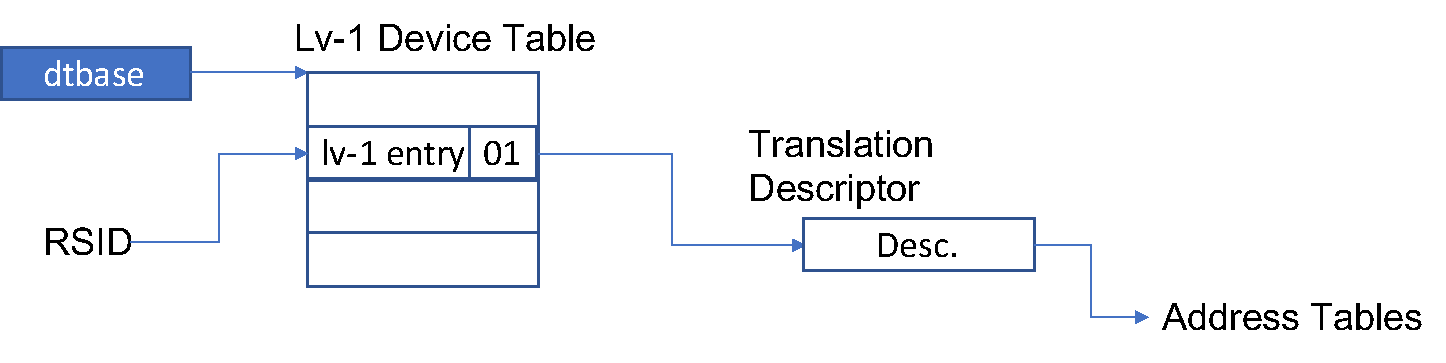
\includegraphics[width=0.95\textwidth]{img/dev_tbl_lookup_short_rsid.pdf}
    \caption{Device table look-up with only RSID and one stage of translation}
    \label{fig:dev_tbl_lookup_rsid_short}
\end{figure}

\begin{figure}[h!t]
    \centering
    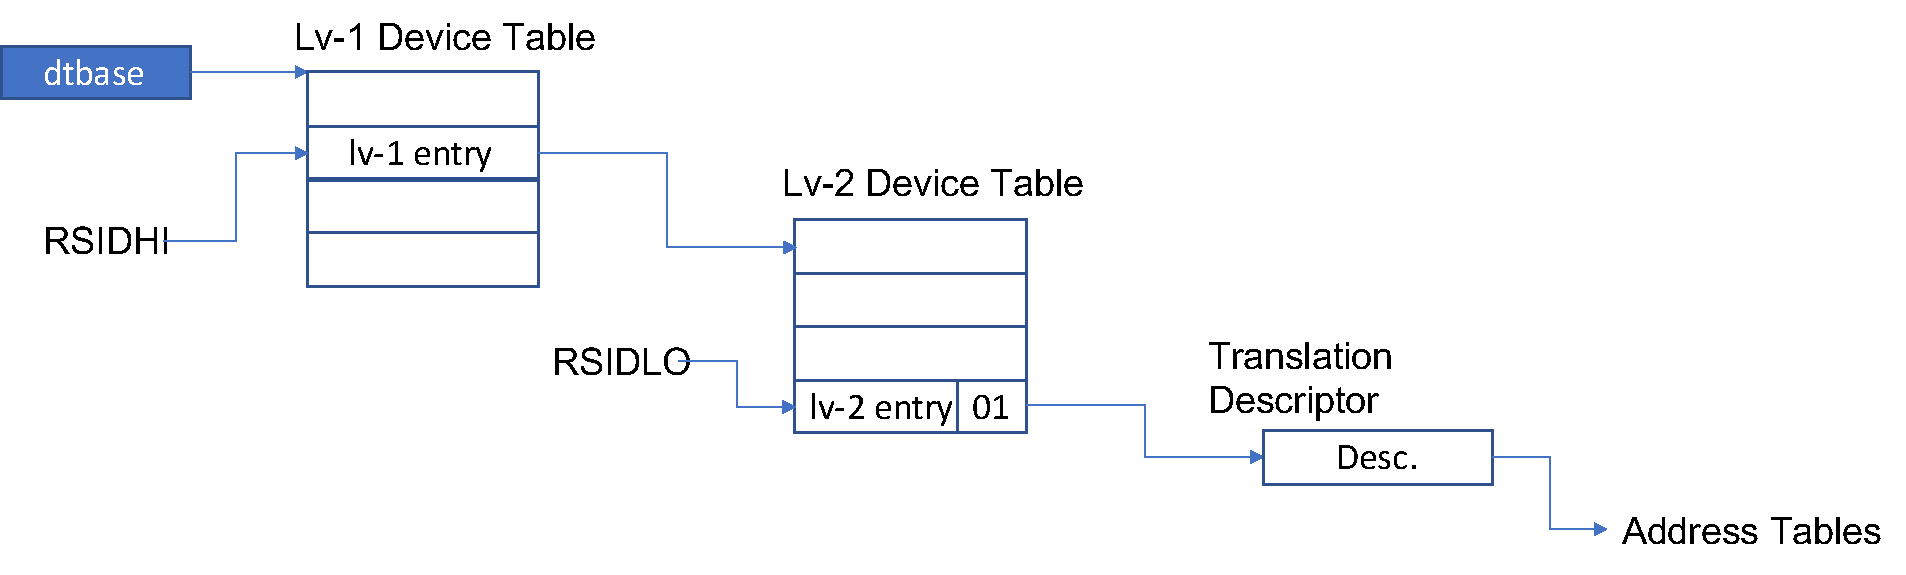
\includegraphics[width=0.95\textwidth]{img/dev_tbl_lookup_bare.pdf}
    \caption{Device table look-up with RSIDHI and RSIDLO and one stage of translation}
    \label{fig:dev_tbl_lookup_bare}
\end{figure}

\begin{figure}[h!t]
    \centering
    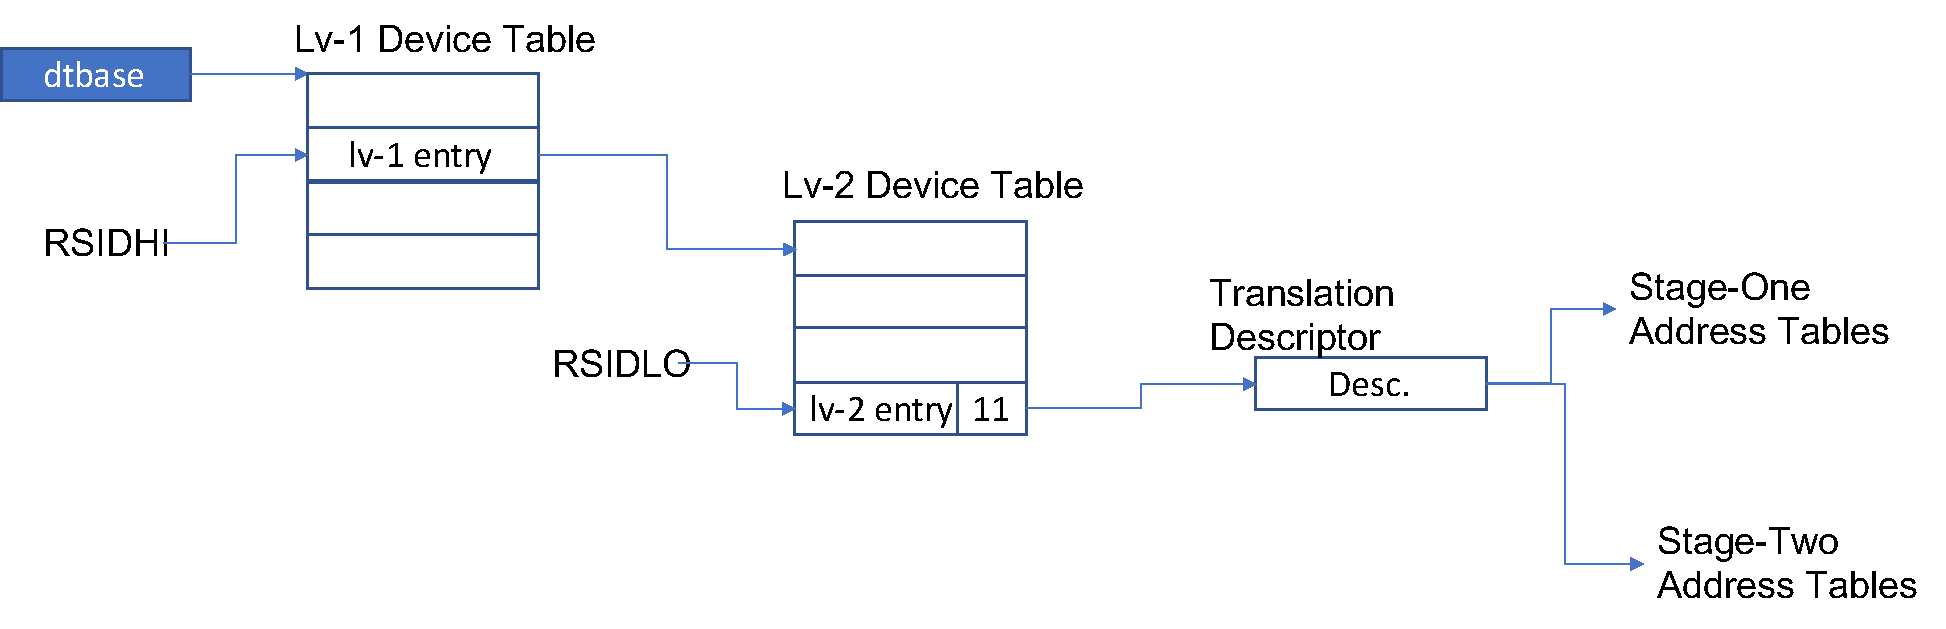
\includegraphics[width=0.95\textwidth]{img/dev_tbl_lookup_two_stage.pdf}
    \caption{Device table look-up when stage-two translation is used.}
    \label{fig:dev_tbl_lookup_two_stage}
\end{figure}


\section{Address Translation}

After a device's configuration is determined, if the device is subject to address
translation, either one-stage or two-stage, The IOMMU performs the address translation
with another set of memory-resident table structure referred to as the \textit{Address
Tables}. During the translation, the IOMMU uses the virtual address and access type of the
memory access and output a physical address or raises a fault for each of the requests.

The address tables are of the same format and have the same alignment requirement as the
translation tables defined in the RISC-V Privileged Architecture.

%TODO: verify this
Besides performing address translations, the IOMMU also grants permissions to the
originating device according to the permission bits in the relevant address table entries.
The IOMMU reports a fault condition if the requested access type is not granted
in the table entries. It is up to the individual originating device to negotiate and setup
proper permission in the IOMMU translation tables. For example, it is up to the driver
code to ensure such permissions are present. 

The IOMMU supports two stages of address translation. Both stages of translation can be
independently enabled and disabled. When the stage-one translation is enabled, it is
typically used by an operating system to assign devices to individual processes. When the
stage-two translation is enabled, it is typically used by the hypervisor to assign devices
to virtual machines. The virtual machines can further enable the stage-one translation to
control the assignment of the device to the processes within the virtual machine.

%\note This design assumes certain identification mechanism for the devices on the
%peripheral buses, such as the bus, device, function numbers of the PCIe bus.


\subsubsection{One Stage Translation}

When the S2MODE is zero, there is only one stage of translation for the corresponding
device. The IOMMU obtains from the device table the root address of the top level
translation table, walks the translation tables and produces an output physical address
for the DMA request.

The translation process when S2MODE = 0 is illustrated in Figure \ref{fig:one-stage-trans}.
Note that the device table lookup is simplified.

\begin{figure}[ht!]
    \centering
    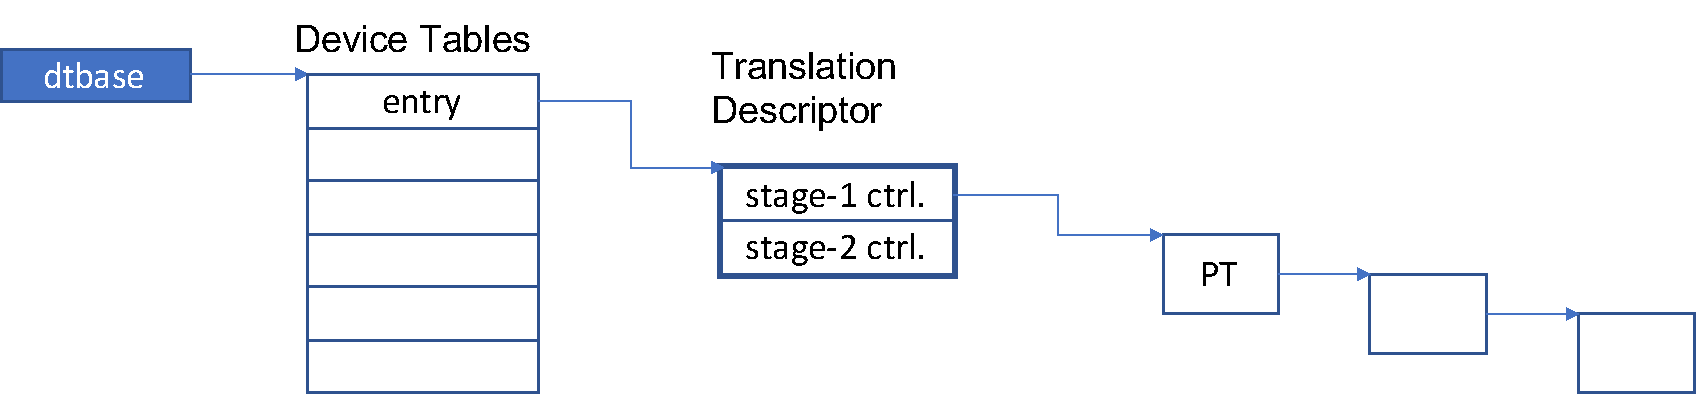
\includegraphics[width=0.95\textwidth]{img/one-stage-trans.pdf}
    \caption{One-Stage Translation}
    \label{fig:one-stage-trans}
\end{figure}

The translation table walk is in principle the same as the page table walk of the MMU,
however, the IOMMU uses the bits in the entries differently. Section \ref{sec:addr_tbl}
lists the bits that are used by the IOMMU.

\subsubsection{Translation with the Second Stage}

When S2MODE is not zero, stage-two translation is enabled. The RPAddr (Register Page
Address) field in the Stage One Control field contains the PPN of the memory space, called
register MMIO page, allocated by the system software, e.g a hypervisor, as the register
MMIO range for the virtual machine. The bytes inside the register MMIO page at the offset
of \dtbase\ contains the guest PPN for the device table defined by the virtual machine,
with which the it may define further translation tables.

\note The system software may also choose to not expose an IOMMU to the virtual machine,
in which case the system software simply provide a dummy register MMIO page for the
virtual machine. All such virtual machines without an IOMMU can share this dummy page,
minimizing memory overhead. \noteend

If the virtual machine does not enable any address translation for the devices assigned to
it, the IOMMU performs translation with only the second stage. Otherwise, the IOMMU
performs both stages of translation, in which the first stage is nested.

The hypervisor is expected to emulate the register MMIO range which include the
\dtbase\ register. When a VM attempts to write to the emulated \dtbase\
register, the hypervisor allocates a physical memory page to hold the values. This
approach keeps the code consistent between the guest VM and the host. 

When the device tables are implemented as MMIO registers, the \dtbase\ register is not
defined. In this case, the memory used to emulate the register MMIO range contains the
device table registers.

The hypervisor is also expected to emulate the command MMIO range. On a write to the
\invltlb\ register, the hypervisor performs the necessary invalidation and
synchronization on the IOMMU TLB. The details of the IOMMU TLB is provided in Section
\ref{sec:tlb}.

\begin{figure}[ht!]
    \centering
    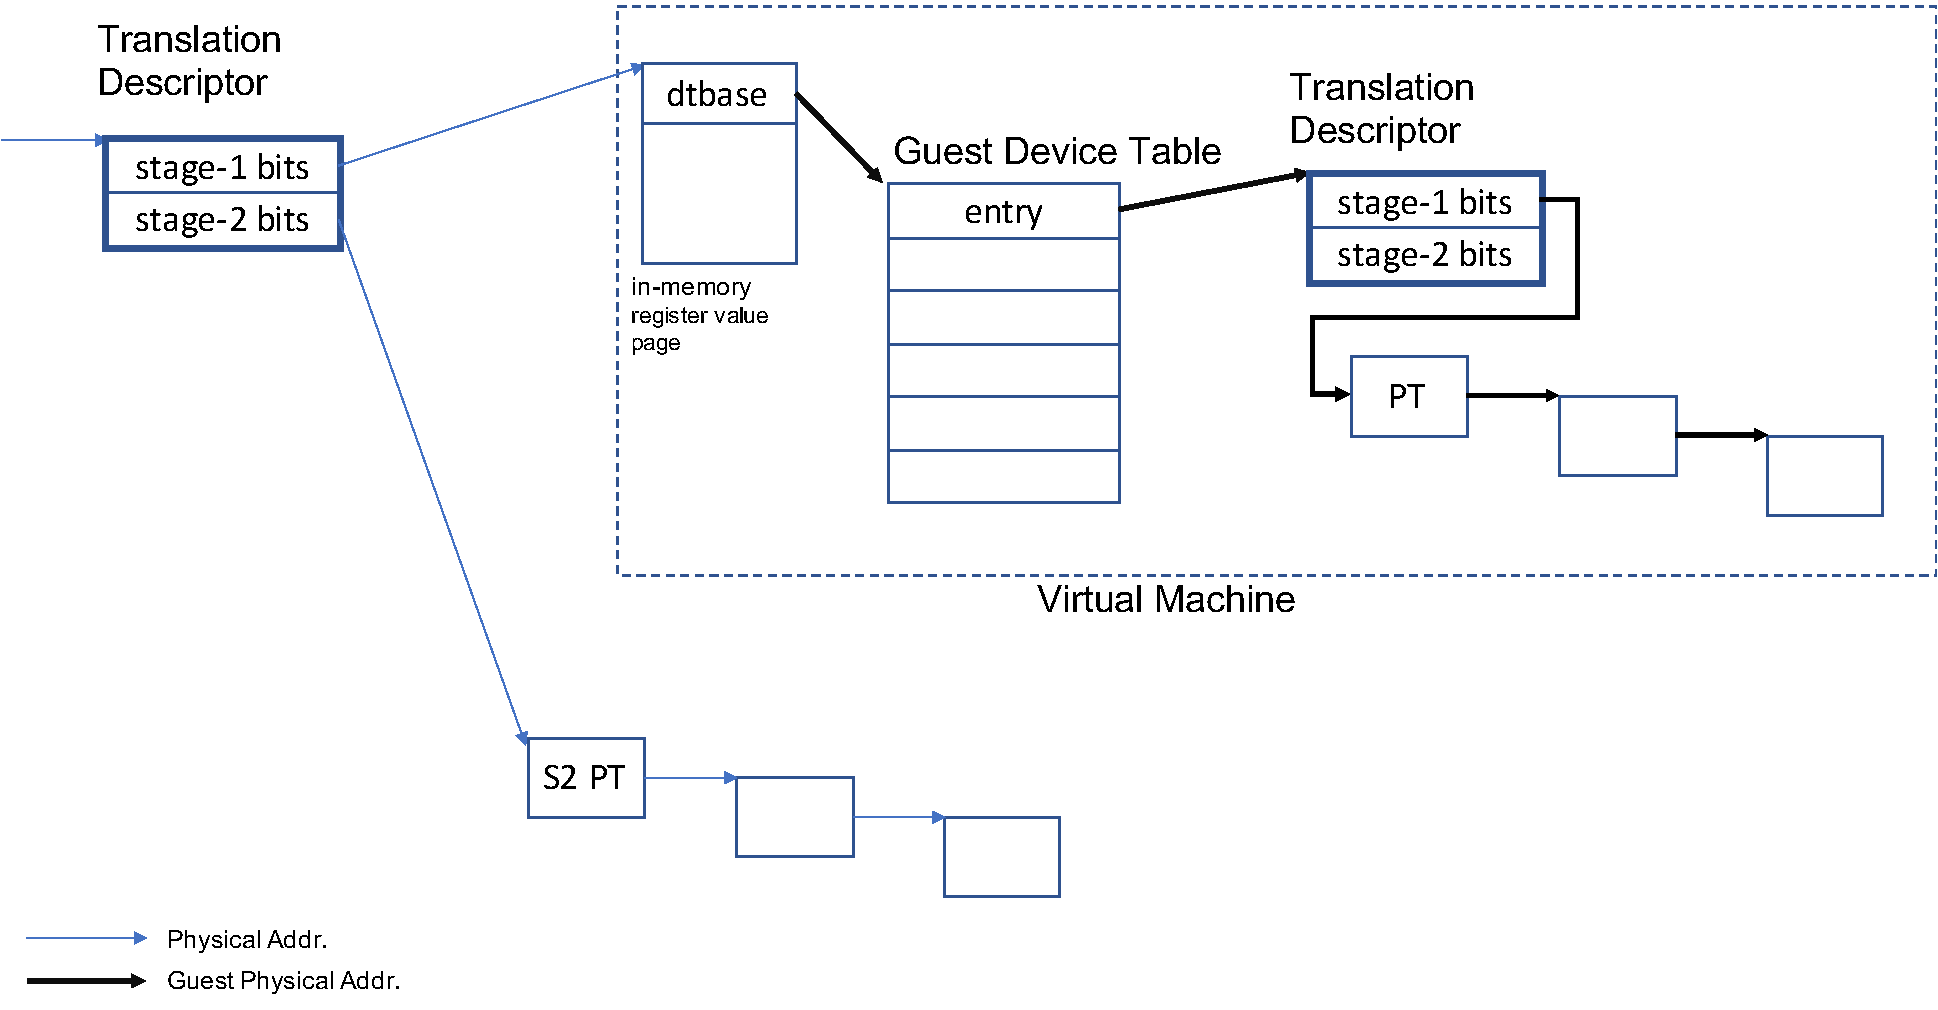
\includegraphics[width=0.95\textwidth]{img/two-stage-trans.pdf}
    \caption{Two-Stage Translation}
    \label{fig:two-stage-trans}
\end{figure}

On a translation request, the IOMMU obtains from the host device table the register page
base address, read the \textit{dtbase} value from the register page, then walks the
address tables pointed to by the guest device table. For each step in the table walk, the
GPAs are translated by the stage-two translation tables pointed to by the host device
table entry. At the end of the table walk, the IOMMU produces a physical address for the
translation request. Figure \ref{fig:two-stage-trans} illustrate the process. Note that
the device table look ups are simplified. 

If there's any fault detected during the table walk, the IOMMU may report the fault as
described in Section \ref{sec:fault} depending on the nature of the fault and the
configuration of the device.


\subsubsection{Update Notification}

Whenever the software updates any the address tables, the register \invltlb\ should be
written to with the RSID of the device whose translation is modified, so that the IOMMU
can perform necessary updates of the internal state. The \invltlb\ register resides in the
command MMIO range. The format of the \invltlb\ register is shown in Figure
\ref{fig:invltlb_reg}.

When the device tables are memory-resident, \invltlb\ is also used to invalid any cached
content inside the IOMMU. However, if the device tables are implemented as MMIO registers,
writing to \invltlb\ is not needed.

A write to the \invltlb\ register is mandatory for the initial setup of the device table.


\begin{figure}[ht!]

    \begin{center}
        \begin{tabular}{@{}T@{}K}
        \instbitrange{63}{\rsidlen} &
        \instbitrange{\rsidlen - 1}{0} \\
        \hline
        \multicolumn{1}{|c|}{Reserved} &
        \multicolumn{1}{ c|}{RSID} \\
        \hline
        63 - \rsidlen & \rsidlen \\
        \end{tabular}
    \end{center}

    \caption{The Format of the \invltlb\ Register}
    \label{fig:invltlb_reg}
\end{figure}

\subsection{Address Translation Procedure}

Below is a sample source code that illustrates the address translation process in C.

\lstinputlisting[language=C]{table_walk.c}


\section{Address Tables}
\label{sec:addr_tbl}

The Address Tables are memory resident structure. They are of the same format as the
MMU page table defined by the RISC-V Privileged Architecture. The IOMMU support
Sv32, Sv39 and Sv48 translation modes. The various page sizes are supported.

Despite of the same format, the IOMMU does not utilize all of the attribute bits in the
table entries. Depending on the features supported, certain bits are ignored by the IOMMU.
The rest of the section provides the details.

The address tables are selected by the look-up in the device tables. The IOMMU walks the
address tables, performing access permission checks along the way and produces a physical
address or raises a fault condition for a particular translation request.

% Sharing of the tables are possible but not without consequences.

\subsection{One-Stage Address Translation}

For one-stage translation, the IOMMU initiate the page table walk from the table pointed
to by the Stage One Control field in the translation descriptor. If the transaction is a read,
the R bit in the leaf address table must be set for the read permission to be granted.
Likewise, if the transaction is a write, both R bit and W bit must be set.

Optionally, if the transaction is of execute type, the X bit must be set in the address
table entries.

\note The exact meaning of the access type is up to the individual device to define. Not
all types of the access are available on a given platform. \noteend

When the originating device distinguishes privileged access and unprivileged access, for
example, an AXI bus that supports distinction between normal or privileged access,
transactions that are marked as privileged are only allowed if the U bit is cleared.
Likewise, transactions that are marked as unprivileged are only allowed if the U bit is
set.

% TODO: not sure about if SUM is needed

If the G bit is set, this translation is global.

The A bit and the D bit are ignored by the IOMMU.

\note For ease of implementation, the A bit and D bit are required to be set. In future
versions, the capability to set the bits by the IOMMU will be considered. \noteend

\subsection{Two-Stage Address Translation}

When the second stage of translation is enabled, all the addresses in the first stage
translation are treated as guest physical addresses and are subject to translation with
the stage-two address tables.

For a translation to succeed in granting the permissions requested in the translation
request during two-stage translation, the permission requested by the device must be
granted in the leaf address table entry in both stages. If the permission is not granted
in any of the stages, the IOMMU raises a fault.

The memory accesses to the entries in the stage-one address tables are treated as read
accesses, therefore, the entries in the last-level stage-two address table that map the
pages that contain the stage-one address table entries must have the R bit set. Otherwise,
the IOMMU raises a fault.

If privileged transaction is supported, the privileged access is only applicable in the
first stage of the translation. The U bit in the stage-one address table entries should be
setup in the same manner as if there is only one stage of translation. The IOMMU raises a
fault when either the access is privileged but the U bit is set, or the access is
unprivileged but the U bit is not set. The memory accesses for the translation of the
stage-one addresses are always considered unprivileged.  Therefore, the U bit in the
second stage address table entries should be set. Otherwise, the IOMMU raises a fault.

The G bit in the stage-two address table entries is ignored by hardware.

\note It is unlikely that the hypervisor assigns a device to be shared by all virtual
machines. \noteend

The A bit and the D bit are ignored by the IOMMU.

\subsubsection{Software Emulation}

To emulate an IOMMU for a virtual machine, the hypervisor allocates pages the size of
register MMIO range and map the pages at the standard address inside the GPA space. The
hypervisor then fills the base address of these pages to the stage-one bits field in the
corresponding device table for that originating device assigned to a virtual machine.

Subsequent operation on the emulated register IOMMU range by the virtual machine does not
cause traps.

When the guest invalidates the IOMMU cache after alteration of the tables, the access to
the command MMIO range is trapped by the host. The host performs the invalidation on
behalf of the guest.


\section{Fault Reporting}
\label{sec:fault}

\subsection{Operation Mode}

The IOMMU operates in one of two modes of error reporting. In \textit{abort-mode}, the
IOMMU terminates the translation and reports the fault to software. It is configurable for
each device whether and how the IOMMU notifies the device that initiated a faulting
transaction.

In \textit{pause-mode}, the IOMMU maintains the state of the faulting transaction before
reporting the fault to software. After handling the fault, the software has the option to
terminate the transaction or resume from the point where the fault occurred.

The mode in which the IOMMU operates in depends on the translation step that the IOMMU is
currently performing. During device table walk, regardless of translation stage, the IOMMU
always operates in abort-mode, albeit the IOMMU still reports the stage during which the
fault is raised. During the address table walk, the IOMMU operates
according to the configuration in the translation descriptor for that device, as specified
in Section \ref{sec:trans_desc}.

\note The device table entries are system-wide configurations, usually set up by the
kernel or the hypervisor. Faults during the device table walk may indicates system-wide
issues, such issues are usually not fixed in a dynamic manner. In contrast, the address
tables are much more dynamic structures, pause-mode allows runtime adjustment to them.
\noteend

In pause-mode, the IOMMU pauses any translation that raises a fault. The in-flight
transaction remains in the state of \textit{in-progress}. The software is required to
resolved the fault and notify the IOMMU that a particular transaction can move forward.
The software has the option to terminate or retry the transaction.

In pause-mode, the IOMMU maintains state information about in-progress transactions for an
\textit{implementation defined} number of devices.  The behavior of the IOMMU when the
storage space for the state information is used up is \textit{implementation defined}. It
is also up to the implementation to specify whether more than one paused transaction
simultaneously is allowed.

\subsubsection{Fault Reporting with One Translation Stages}

When the IOMMU is only performing one stage of translation, it operates in abort-mode when
walking the device tables. It works in the mode configured by the translation descriptor
when walking the address tables.

\subsubsection{Fault Reporting with Two Translation Stages}

When the IOMMU is performing two stages of translation, the behavior when the IOMMU is
walking in the stage-2 translation structures, i.e., the host device tables and the
stage-2 address tables, is the same as when the IOMMU is only performing one stage of
translation. When the IOMMU is walking the stage-1 structures, the default behavior is the
same as the stage-2 behavior, however, the host can override the behavior in the
translation descriptor.


\subsection{Fault Reporting Registers}

The IOMMU generates an interrupt when a fault is raised during the translation. A command
MMIO range register \iommuinten\ is provided to enable the interrupt from the IOMMU. When
the E bit is one, the interrupt is enabled. When the register is zero, the interrupt is
suppressed. The format of the \iommuinten\ register is shown in Figure
\ref{fig:iommuinten}.

\begin{figure}[h!t]
    \begin{center}
        \begin{tabular}{@{}Jc@{}I}
    \instbitrange{63}{1} &
    \instbit{0} \\
    \hline
    \multicolumn{1}{|c|}{Reserved} &
    \multicolumn{1}{c| }{E} \\
    \hline
    63 & 1 \\

    \end{tabular}
    \end{center}

    \caption{The \iommuinten\ Register}
    \label{fig:iommuinten}
\end{figure}


\note The capability to control the interrupt is for batch process of possible multiple
faults that occurs at the same time. The handler can suppress the interrupt during the
handling, and checks if there are other faults before returning, a known technique. \noteend

The interrupt number is provided in the register MMIO range register called \iommuintno.
The hardware may choose to hardwire this register. In the case that the platform is
equipped with an AIA interrupt controller, this interrupt number is the minor entity
assigned to the IOMMU in any way that is appropriate. The format of this register is shown
in Figure \ref{fig:iommuintno}.

\begin{figure}[h!t]
    \begin{center}
        \begin{tabular}{@{}Jc}
    \instbitrange{63}{0} \\
    \hline
    \multicolumn{1}{| c | }{IntNo} \\
    \hline
    64 \\

    \end{tabular}
    \end{center}

    \caption{The \iommuintno\ Register}
    \label{fig:iommuintno}
\end{figure}


\note The platform can choose to implement the interrupt with any implementation defined
approach. For example, if AIA is implemented, the IOMMU may generate an MSI to the IMSIC
of a hart. If the platform uses the PLIC, the interrupt can be reported as interrupt
routed through the PLIC. \noteend

The read-only register in the register MMIO range \iommucause\, shown in Figure
\ref{fig:iommucause}, provide the code for the
fault reason. Table \ref{tbl:fault_reasons} provides all the reason codes. 

The RSID field provide the ID of the device that raised the fault. The V bit of \iommucause\
indicates if there is a pending fault that needs to be handled.  A read to \iommucause\
has the side-effect of clearing the V bit if there is no other pending fault.

\begin{figure}[h!t]
    \begin{center}
        \begin{tabular}{@{}I@{}M@{}M@{}S}
    \instbit{63} &
    \instbitrange{62}{RSIDLEN + 16} &
    \instbitrange{RSIDLEN + 15}{16} &
    \instbitrange{15}{0} \\
    \hline
    \multicolumn{1}{|c|}{V} &
    \multicolumn{1}{c|}{Reserved} &
    \multicolumn{1}{c|}{RSID} &
    \multicolumn{1}{c| }{Cause} \\
    \hline
    1 &  & RSIDLEN & 16 \\

    \end{tabular}
    \end{center}

    \caption{The \iommucause\ Register}
    \label{fig:iommucause}
\end{figure}

The read-only register in the register MMIO range \ftval\ provide additional data for the
relevant fault, e.g. the address of the entry that caused the fault. The \ftval\ register
is shown in Figure \ref{fig:ftval}.

\begin{figure}[h!t]
    \begin{center}
        \begin{tabular}{@{}Jc}
    \instbitrange{63}{0} \\
    \hline
    \multicolumn{1}{| c | }{Value} \\
    \hline
    64 \\

    \end{tabular}
    \end{center}

    \caption{The \ftval\ Register}
    \label{fig:ftval}
\end{figure}

Once a request is paused, the IOMMU remains inactive for the device that caused the fault.
It returns failure for all subsequent memory requests from the faulting device until a
write is performed to the command MMIO range register \resume\ with the RSID of the
faulting device. The IOMMU then proceed with the previously-faulted transaction caused by
the device with the written RSID. If a RSID is written, however, there is no such
transaction that previously faulted, the IOMMU ignores the write.

\begin{figure}[h!t]
    \begin{center}
        \begin{tabular}{@{}I@{}M@{}N}
    \instbit{63} &
    \instbitrange{62}{RSIDLEN} &
    \instbitrange{RSIDLEN - 1}{0} \\
    \hline
    \multicolumn{1}{|c|}{T} &
    \multicolumn{1}{c|}{Reserved} &
    \multicolumn{1}{c|}{RSID} \\
    \hline
    1 & & RSIDLEN \\

    \end{tabular}
    \end{center}

    \caption{The \resume\ Register}
    \label{fig:resume}
\end{figure}


The T bit in the \resume\ register is provided for software to specify the type of
resumption.  A value of zero means to terminate the transaction. A value of one means to
retry the faulting translation. When the IOMMU is notified to terminate the transaction,
it returns an error to the device that initiates the transaction. It is up to the device
to decide if it is necessary to re-initiate the same transaction. When the IOMMU is
notified to resume the transaction, the IOMMU restarts the entire translation process as
if it is a newly received transaction.

\note When a fault occurs, there are usually other device-specific operations needed to
completely handle the fault. It is up to the specific device and the corresponding device
driver to address them. \noteend

\subsection{Direct Delivery of Fault Interrupt to VM}

The IOMMU maybe designed to work with two types of interrupt systems, the legacy PLIC and
the AIA.

When PLIC is used, a separate interrupt is not provided when the two-stage translation is supported.
The reasoning is that if such an interrupt is provided, the hypervisor might attempt to
directly assign the interrupt for reporting stage-one translation faults to a guest VM.
However, currently the \ftval\ register is in the register MMIO range, the hypervisor
needs to move this data to the memory page that emulates the register MMIO range for the
IOMMU for the guest anyway. A trap is inevitable. Therefore an extra interrupt number is
not needed.

When AIA is used, the IOMMU does have the option to directly deliver
virtual interrupts when a fault is encountered during the first stage of translation. It
may do so by implementing the MSI translation tables defined by the AIA and send MSIs
directly to the IMSIC registers designated to the VM.

To minimize number of traps the VM encounters during handling of the interrupt, in
addition to update the \ftval\ register, the IOMMU
also needs to perform a write to the 8-bytes starting of the offset of the \ftval\
register within the register MMIO range inside the register MMIO page. The write provide
the same value that is written into the \ftval\ register. Subsequently, the VM does not
trap when reading from the emulated register MMIO range.

%how about interrupt control? that still traps?


\begin{table}
    \centering
    \begin{tabular}{| p{0.05\linewidth} | p{0.95\linewidth} |}
        \hline
         Code  & Reason \\
        \hline
         1      & Reserved bits are not zero in the device table entries \\
        \hline
         2      & The S bit is set in a device table entry, however, the translation descriptor contains zeros for S2MODE field \\
        \hline
         21     & R bit is not set in the stage-one address table entry for a read transaction \\
        \hline
         22     & W bit is not set in the stage-one address table entry for a write transaction  \\
        \hline
         23     & X bit and R bit are not both set in the stage-one address table entry for an execute transaction \\
        \hline
         24     & U bit is set in the stage-one address table entry for a privileged transaction \\
        \hline
         25     & U bit is not set in the stage-one address table entry for an unprivileged transaction \\
        \hline
         26     & A bit and D bit are not both set in a stage-one address table entry \\
        \hline
         51    & R bit is not set in the stage-two address table entry for a read transaction \\
        \hline
         52    & W bit is not set in the stage-two address table entry for a write transaction \\
        \hline
         53    & X bit and R bit are not both set in the stage-two address table entry for an execute transaction \\
        \hline
         54    & U bit is set in the stage-two address table entries \\
        \hline
    \end{tabular}
    \caption{List of Fault Reasons During Address Table Walk}
    \label{tbl:fault_reasons}
\end{table}


\section{TLB}
\label{sec:tlb}

The translation process involves a number of memory read, which may incur a long latency.
The IOMMU can optionally include a Translation Look-aside Buffer(TLB) to cache
translation table walk results. The number of the entry in the TLB is implementation
defined.

The TLB entries are tagged by the VMID field and the ASID field in the translation
descriptor. If a device is only subject to one stage of translation, the VMID is assumed
to be zero. If a device is only subject to stage two translation, the ASID is assumed to
be zero.

The IOMMU provides the invalidate register \invltlb\ to flush the designated entry in
the TLB. The \invltlb\ register is in the command MMIO range.

A write to the \invltlb\ with the value of the RSID of a device invalidates the cached
content of the table structures for that device.

% Prefetching for lower latency

% TODO: can it cache device table entries?

\subsection{TLB Organization}

The TLB implemented by the IOMMU could be of a single or multiple hierarchy, and could be
a monolithic or distributed configuration. However, from the software's point of view, the
IOMMU does not expose the internal structure of the TLB and behave as if there is no TLB.
It is up to the implementation to ensure that all subcomponents of the TLB operate in a
coherent manner.

\subsection{Other Caching Consideration}

The address translation by IOMMU involves a potentially large number of memory accesses,
which may incur a large amount of delay when the TLB misses. It is recommended to
implement further caching mechanism to minimize the delay during walking the
memory-resident table structures. The implementation is required to maintain the
coherency of the caches.

\note One straightforward design is simply caching the most-recently used table entry.
\noteend


\section{Ordering Considerations}

Since the IOMMU works in the transparent configuration, it is required to behave as much
as how a wire behave. In addition, the IOMMU conforms to the ordering constraint of the
bus it is interfacing with. For example, AXI bus requires that ``all transactions with a
given ID must ordered, but there is no restriction on the ordering of transactions with
different IDs''. The IOMMU is therefore required to maintain order only within a given
RSID.

This implies that if the IOMMU supports pause-mode of fault reporting and if any of the
transactions with a given ID faults, all subsequent transactions should be suspended until
the fault is handled. This requirement implies that the IOMMU implementation should be
able to buffer all subsequent transactions before the fault is handled. The number of
transactions that need to be buffered is highly implementation dependent, and is left for
each implementation to decide.

Handling the fault may result in canceling the transaction either directly by the IOMMU or
by the software, in this case, the IOMMU returns error for all subsequent transactions
with the same RSID.


\section{Working with IOPMP}

The IOMMU and the IOPMP complement each other and provide in-depth defense against
malicious DMA request by malicious devices.

The current design of IOMMU has full control over the permission granted to each device.
However,when the device table's V bit is cleared, the device obtains direct access to
physical memory.Furthermore, future version of the IOMMU is expected to work with the
Address Translation Service (ATS) of the PCI-Express. ATS allows devices to mark DMA
requests as 'translated' so that the IOMMU simply passes the requests to the
interconnects. This is a potential security hole because a malicious device can always
mark any DMA requests as 'translated'.

In this case, the IOMMU can pair with the IOPMP which specify which physical address range
is allowed for a given device, even if the request is marked as translated, the IOPMP will
be able to deny the access.

\subsection{Built-in IOPMP}

%TODO
The translation descriptor can be optionally extended with the pmpcfg and pmpaddr field
for that device. They follow the same format as defined in the PMP in the RISC-V
Privileged Architecture. After the translation is complete, the output physical address is
compared with the pmpcfg and pmpaddr entries for further checks. 


\section{PCI-Express Extension}

The IOMMU can optionally implement a set of features to support PCIe based systems, such
as desktop computers and servers. The PCI-Express specification describes such a component
as a Translation Agent (TA), which serves as the model that this IOMMU specification is
conforming to.

\subsection{Device Identification}

\subsection{Device Table Extension}

\subsection{Two-stage Translation}

\section{List of Registers}

\subsection{Register MMIO Range}
\begin{enumerate}
    \item \iommucap
    \item \rsiddiv
    \item \ersiddiv
    \item \dtbase
    \item \ftval
\end{enumerate}

\subsection{Command MMIO Range}

\begin{enumerate}
    \item \iommucapen
    \item \iommuinten
    \item \invltlb
    \item \resume
\end{enumerate}



\end{document}
